% D036 canonical bounded edition generated from frozen packet records.
% Controlling authority SHA-256: 278125A52E24555349D7A7B56A5EE828FF2BC1952F752969B20E7BDD8228A74D.
\documentclass[10pt,a4paper]{article}
\usepackage{fontspec}
\usepackage{unicode-math}
\setmainfont{Latin Modern Roman}
\setsansfont{Latin Modern Sans}
\setmonofont{Latin Modern Mono}
\setmathfont{Latin Modern Math}
\usepackage{amsmath,mathtools,graphicx,adjustbox,geometry,microtype,hyperref,bookmark}
\usepackage[english]{babel}
\geometry{top=13mm,bottom=13mm,left=13mm,right=13mm}
\hypersetup{hidelinks,pdftitle={The Fundamental Group of the Complement of a Plane Curve},pdfauthor={Pierre Deligne},pdfcreator={D036 canonical XeLaTeX builder},pdfproducer={XeTeX},pdfcreationdate={D:19791101000000Z},pdfmoddate={D:19791101000000Z}}
\pagestyle{empty}
\setlength{\parindent}{0pt}
\setlength{\parskip}{0.10em}
\setlength{\emergencystretch}{3em}
\tolerance=2500
\hfuzz=1.5pt
\raggedbottom
\begin{document}
\fontsize{8.05}{9.15}\selectfont
\noindent\begin{adjustbox}{max totalsize={\textwidth}{0.945\textheight},center}
\begin{minipage}{\textwidth}
\noindent\hfill\scriptsize Authority physical page 1 / printed folio 543-01\par\normalsize
\begin{center}BOURBAKI SEMINAR\\32nd year, 1979/80, no. 543\\November 1979\end{center}
\begin{center}\bfseries THE FUNDAMENTAL GROUP OF THE COMPLEMENT\\OF A PLANE CURVE HAVING ONLY ORDINARY\\DOUBLE POINTS IS ABELIAN\end{center}
\begin{center}[after W. FULTON]\end{center}
\begin{center}by Pierre DELIGNE\end{center}
\noindent Introduction\par\smallskip
\noindent THEOREM 1.- Let C \ensuremath{⊂} \ensuremath{ℙ^2}(\ensuremath{ℂ}) be a plane curve whose only singularities are double points with distinct tangents. Then the fundamental group of \ensuremath{ℙ^2}(\ensuremath{ℂ}) - C is abelian.\par\smallskip
\noindent This theorem was stated by Zariski in 1929 ([8]). See also [9], Ch. VIII. His proof used Severi's theorem, according to which the space of irreducible plane curves of a given degree having a given number of double points is irreducible (Vorlesungen über algebraische Geometrie, 1921, Anhang F). It is still unknown whether Severi's assertion is true or false.\par\smallskip
\noindent The \ensuremath{π₁} considered in the theorem is the genuine fundamental group, the topologists' one. If \ensuremath{ℂ} is replaced by an arbitrary algebraically closed field k of characteristic 0, the same statement holds for the algebraic fundamental group, the one classifying étale coverings: the Lefschetz principle reduces us to assuming k = \ensuremath{ℂ}, in which case the algebraic fundamental group is the profinite completion of the genuine fundamental group. In arbitrary characteristic one has the variant:\par\smallskip
\noindent THEOREM 2 (Fulton [3]).- Let k be an algebraically closed field and, over k, let C \ensuremath{⊂} \ensuremath{ℙ^2} be a plane curve whose only singularities are double points with distinct tangents. Then the tame fundamental group of \ensuremath{ℙ^2} - C is abelian.\par\smallskip
\noindent In other words, coverings (in the sense of 0.2) of \ensuremath{ℙ^2}, ramified only along C and tamely ramified, are abelian. Recall that tameness of the ramification is tested after base change from \ensuremath{ℙ^2} to its localizations at the generic points of the irreducible components of C. These localizations are traits (spectra of discrete valuation rings).\par\smallskip
\noindent Suppose k has characteristic p > 0. If C is as in Theorem 2, there always exists in relative projective space \ensuremath{ℙ^2} over Spec(W(k)) a relative normal-crossings divisor \ensuremath{\widetilde{C}} whose special fiber is C (see, for example, Mumford, Appendix to Ch. VIII of [9]). This makes it possible to deduce Theorem 2 from Theorem 1 by a specialization argument.\par\smallskip
\end{minipage}
\end{adjustbox}
\newpage
\noindent\begin{adjustbox}{max totalsize={\textwidth}{0.945\textheight},center}
\begin{minipage}{\textwidth}
\noindent\hfill\scriptsize Authority physical page 2 / printed folio 543-02\par\normalsize
\noindent Once one knows that \ensuremath{π₁}(\ensuremath{ℙ^2}(\ensuremath{ℂ}) - C) is abelian, homological arguments immediately give its structure: if C is the union of irreducible curves of degrees d\ensuremath{₁}, ..., \ensuremath{d_r}, then \ensuremath{π₁}(\ensuremath{ℙ^2}(\ensuremath{ℂ}) - C) is the quotient of \ensuremath{ℤ^r} by the subgroup generated by the element (d\ensuremath{₁}, ..., \ensuremath{d_r}).\par\smallskip
\noindent In his proof of Theorem 2, Fulton uses, on the one hand, methods introduced by Abhyankar [1] to prove the special case of Theorem 2 in which the irreducible components of C are assumed smooth - methods very clearly presented here by Serre ([7]) - and, on the other hand, Theorem 3 below. An analysis of the proof then enabled the expositor to give a variant yielding Theorem 1.\par\smallskip
\noindent Abhyankar and Fulton both use instances of the principle that, in algebraic geometry, what is very mobile is connected. Let C \ensuremath{⊂} \ensuremath{ℙ^2} be as in Theorem 2, let D be an irreducible component of C, and let f : X \ensuremath{→} \ensuremath{ℙ^2} be a covering ramified only along C and tamely ramified. Since D \ensuremath{⊂} \ensuremath{ℙ^2} is very mobile, \ensuremath{f^{-1}}(D) is connected. More precisely, the divisor D \ensuremath{⊂} \ensuremath{ℙ^2} is ample, hence the divisor \ensuremath{f^{-1}}(D) \ensuremath{⊂} X is also ample because f is finite, and one applies Bertini. By a local study of f, Abhyankar shows that if D is smooth then (\ensuremath{f^{-1}}(D))red is smooth as well, and concludes that \ensuremath{f^{-1}}(D) is irreducible.\par\smallskip
\noindent In the general case, let g : \ensuremath{\widetilde{D}} \ensuremath{→} D be the normalization of D. The same local study shows that the reduced fiber product (X \ensuremath{×_{ℙ^2}} \ensuremath{\widetilde{D}})red is smooth. It is therefore the normalization of \ensuremath{f^{-1}}(D). If it can be shown to be connected, it follows that \ensuremath{f^{-1}}(D) is irreducible, and one can repeat the end of Abhyankar's proof as presented in [7].\par\smallskip
\noindent Recall the definition of the fiber product: if h : X \ensuremath{×} \ensuremath{\widetilde{D}} \ensuremath{→} \ensuremath{ℙ^2} \ensuremath{×} \ensuremath{ℙ^2} is the product of the maps f : X \ensuremath{→} \ensuremath{ℙ^2} and g : \ensuremath{\widetilde{D}} \ensuremath{→} D \ensuremath{⊂} \ensuremath{ℙ^2}, then the fiber product X \ensuremath{×_{ℙ^2}} \ensuremath{\widetilde{D}} is the inverse image \ensuremath{h^{-1}}(\ensuremath{Δ}) of the diagonal. Since \ensuremath{ℙ^2} has many automorphisms, the diagonal \ensuremath{Δ} \ensuremath{⊂} \ensuremath{ℙ^2} \ensuremath{×} \ensuremath{ℙ^2} is very mobile, and \ensuremath{h^{-1}}(\ensuremath{Δ}) is connected. This completes the proof. More precisely, one applies to h the special case r = 2, m = 2 of the following theorem:\par\smallskip
\noindent THEOREM 3 (W. Fulton and J. Hansen [4]).- Let P = \ensuremath{(ℙ^m)^r} be the product of r copies of projective space \ensuremath{ℙ^m}, let \ensuremath{δ} be the diagonal map from \ensuremath{ℙ^m} to P, let \ensuremath{Δ} = \ensuremath{δ}(\ensuremath{ℙ^m}) be the diagonal, let Z be a complete irreducible variety, let h : Z \ensuremath{→} P, let n = dim h(Z), and let c = (r - 1)m be the codimension of \ensuremath{Δ} in P. If n - c \ensuremath{≥} 1, then \ensuremath{h^{-1}}(\ensuremath{Δ}) is connected.\par\smallskip
\noindent This theorem has many other applications, for which I refer to [4] and to the article of T. Gaffney and R. Lazarsfeld [5].\par\smallskip
\noindent At the end of this introduction, we explain by an example the method used to transpose Fulton's proof of Theorem 2 into a proof\par\smallskip
\end{minipage}
\end{adjustbox}
\newpage
\noindent\begin{adjustbox}{max totalsize={\textwidth}{0.945\textheight},center}
\begin{minipage}{\textwidth}
\noindent\hfill\scriptsize Authority physical page 3 / printed folio 543-03\par\normalsize
\noindent of Theorem 1. The example is this: how to transpose Abhyankar's arguments to prove Theorem 1 in the special case where C is smooth (hence irreducible).\par\smallskip
\noindent Let U be a tubular neighborhood of C in \ensuremath{ℙ^2}(\ensuremath{ℂ}), let U* = U - C, and let u \ensuremath{∈} U*. For every covering f : X \ensuremath{→} \ensuremath{ℙ^2}(\ensuremath{ℂ}) ramified only along C, one has\par\smallskip
\noindent (\ensuremath{f^{-1}}(C) connected) \ensuremath{⇔} (\ensuremath{f^{-1}}(U) connected) \ensuremath{⇔} (\ensuremath{f^{-1}}(U*) connected).\par\smallskip
\noindent The key result - that for every covering X the curve \ensuremath{f^{-1}}(C) is connected - is therefore equivalent to the following: for every finite quotient H of \ensuremath{π₁}(\ensuremath{ℙ^2}(\ensuremath{ℂ}) - C,u), the composite map\par\smallskip
\noindent \ensuremath{π₁}(U*,u) —j*\ensuremath{→} \ensuremath{π₁}(\ensuremath{ℙ^2}(\ensuremath{ℂ}) - C,u) \ensuremath{→} H\par\smallskip
\noindent is surjective. A Morse-theoretic argument proves more: the map j* : \ensuremath{π₁}(U*,u) \ensuremath{→} \ensuremath{π₁}(\ensuremath{ℙ^2}(\ensuremath{ℂ}) - C,u) is surjective.\par\smallskip
\noindent After choosing a Riemannian metric on \ensuremath{ℙ^2}(\ensuremath{ℂ}), for \ensuremath{ε} > 0 sufficiently small one may take U to be the image under the exponential map exp of the subbundle of balls of radius \ensuremath{ε} in the normal bundle of C in \ensuremath{ℙ^2}(\ensuremath{ℂ}). For \ensuremath{ε} sufficiently small, exp identifies U* with an oriented punctured-disk bundle over C, giving an exact sequence\par\smallskip
\noindent \ensuremath{ℤ} \ensuremath{→} \ensuremath{π₁}(U*,u) \ensuremath{→} \ensuremath{π₁}(C,\ensuremath{\bar{u}}) \ensuremath{→} 1\par\smallskip
\noindent (\ensuremath{\bar{u}} is the image of u). The image of \ensuremath{ℤ} is central; the image of 1 \ensuremath{∈} \ensuremath{ℤ} is represented by a small loop \ensuremath{γ} going once around C in the positive direction.\par\smallskip
\noindent Since j* is surjective, \ensuremath{γ} also defines a central element of \ensuremath{π₁}(\ensuremath{ℙ^2}(\ensuremath{ℂ}) - C,u). The quotient of \ensuremath{π₁}(\ensuremath{ℙ^2}(\ensuremath{ℂ}) - C,u) by the normal subgroup generated by \ensuremath{γ} (in this case, the cyclic subgroup generated by \ensuremath{γ}) is \ensuremath{π₁}(\ensuremath{ℙ^2}(\ensuremath{ℂ}),u) = \{e\}, and the special case of the theorem under consideration follows.\par\smallskip
\noindent 0. Terminology\par\smallskip
\noindent 0.1. Connected means connected and nonempty. The same convention applies to irreducible.\par\smallskip
\noindent 0.2. A covering of a scheme S, assumed normal and connected, is a morphism f : T \ensuremath{→} S whose source T is normal and connected and whose restriction to a dense open subset of T is étale.\par\smallskip
\noindent 0.3. Throughout the rest of this exposition we work over \ensuremath{ℂ}. We shall write simply \ensuremath{ℙ^n} for \ensuremath{ℙ^n}(\ensuremath{ℂ}). All schemes considered are assumed separated.\par\smallskip
\end{minipage}
\end{adjustbox}
\newpage
\noindent\begin{adjustbox}{max totalsize={\textwidth}{0.945\textheight},center}
\begin{minipage}{\textwidth}
\noindent\hfill\scriptsize Authority physical page 4 / printed folio 543-04\par\normalsize
\noindent 1. Theorems of Lefschetz and Bertini type\par\smallskip
\noindent The special case of 1.1 below in which Z \ensuremath{⊂} \ensuremath{ℙ^n} is the complement of a hypersurface is proved by Hamm and Lê [6], using Morse theory. Our aim in this section is to deduce from it the variant 1.6 of Theorem 3.\par\smallskip
\noindent Assertion 1.1.- Let Z \ensuremath{⊂} \ensuremath{ℙ^n} be a nonempty Zariski-open subset. If H is a general hyperplane, the natural map \ensuremath{π_i}(Z \ensuremath{∩} H) \ensuremath{→} \ensuremath{π_i}(Z) is bijective for i < n - 1 and surjective for i = n - 1.\par\smallskip
\noindent Assertion 1.1 is stated in [2], but Cheniot's proof covers only the case in which the complement of Z has codimension \ensuremath{≥} 2. Under this hypothesis, Z and Z \ensuremath{∩} H are simply connected, and it is harmless to work, as he does, with the \ensuremath{H_i} rather than the \ensuremath{π_i}. The case i = 1 can also be deduced from [6] or [2 bis].\par\smallskip
\noindent Recall that the adjective “general,” qualifying an element H of an irreducible algebraic variety S (here the dual projective space \ensuremath{ℙ^n}\ensuremath{∨}), is a quantifier. It means that there exists a nonempty (hence dense) Zariski-open subset S' of S such that for every H in S', ....\par\smallskip
\noindent 1.2.- Let Y \ensuremath{⊂} \ensuremath{ℙ^n} \ensuremath{×} \ensuremath{ℙ^n}\ensuremath{∨} be the space of pairs (z,H) such that z \ensuremath{∈} Z and z \ensuremath{∈} H. The isotopy theorem, applied to the second projection pr\ensuremath{₂} : Y \ensuremath{→} \ensuremath{ℙ^n}\ensuremath{∨}, gives a nonempty Zariski-open subset U of \ensuremath{ℙ^n}\ensuremath{∨} over which Y is a topologically locally trivial fiber space. It is enough to take U to be the set of hyperplanes transverse to the strata of an algebraic Whithney stratification of the complement of Z in \ensuremath{ℙ^n}. Locally over U, after choosing a local trivialization of this fiber space, the inclusion Z \ensuremath{∩} H = pr\ensuremath{₂^{-1}}(\{H\}) into Z appears as a continuously H-dependent map from a fixed space into Z. Thus the conclusion of 1.1 can hold for one H in U only if it holds for all of them, and 1.1 is equivalent to saying that it holds for every H in U.\par\smallskip
\noindent Suppose that Z depends on parameters: take an irreducible scheme S and an open subset Z of S \ensuremath{×} \ensuremath{ℙ^n}; set pr\ensuremath{₂} pr\ensuremath{₁^{-1}}(\{s\}) = Z(s), and assume every Z(s) is nonempty. Let Y \ensuremath{⊂} S \ensuremath{×} \ensuremath{ℙ^n} \ensuremath{×} \ensuremath{ℙ^n}\ensuremath{∨} be the space of triples (s,z,H) such that z \ensuremath{∈} Z(s) and z \ensuremath{∈} H. The isotopy theorem, applied to the projection of Y onto S \ensuremath{×} \ensuremath{ℙ^n}\ensuremath{∨} (respectively, of Z onto S), gives a nonempty Zariski-open subset U of S \ensuremath{×} \ensuremath{ℙ^n}\ensuremath{∨} (respectively V of S) over which Y (respectively Z) is a topologically locally trivial fiber space.\par\smallskip
\noindent As above, if s \ensuremath{∈} V and (s,H) \ensuremath{∈} U, the conclusion of 1.1 holds for Z(s) and H. This parameterized variant of 1.1 will be used implicitly in the proof of 1.4.\par\smallskip
\noindent I conjecture more generally:\par\smallskip
\noindent Conjecture 1.3.- Let Z be smooth and connected of dimension n, let f : Z \ensuremath{→} \ensuremath{ℙ^N} be a morphism with finite fibers, let c be an integer, and let L be a linear subspace of \ensuremath{ℙ^N} of\par\smallskip
\end{minipage}
\end{adjustbox}
\newpage
\noindent\begin{adjustbox}{max totalsize={\textwidth}{0.945\textheight},center}
\begin{minipage}{\textwidth}
\noindent\hfill\scriptsize Authority physical page 5 / printed folio 543-05\par\normalsize
\noindent codimension c, with n* = n - c. Choose a Riemannian metric on \ensuremath{ℙ^N}, and let V(\ensuremath{ε}) be the set of points p of \ensuremath{ℙ^N} such that d(p,L) < \ensuremath{ε}. Then, for \ensuremath{ε} sufficiently small, the natural map\par\smallskip
\noindent \ensuremath{π_i}(\ensuremath{f^{-1}}(V(\ensuremath{ε}))) \ensuremath{→} \ensuremath{π_i}(Z)\par\smallskip
\noindent is bijective for i < n* and surjective for i = n*.\par\smallskip
\noindent For general L, the inclusion of \ensuremath{f^{-1}}(L) into \ensuremath{f^{-1}}(V(\ensuremath{ε})) is, for \ensuremath{ε} sufficiently small, a homotopy equivalence: 1.3 is indeed a generalization of 1.1.\par\smallskip
\noindent If f is no longer assumed quasi-finite, and if the set of points of \ensuremath{ℙ^N} where the fiber of f has dimension k has dimension \ensuremath{φ}(k), then n* should be redefined as\par\smallskip
\noindent n* = 2 dim Z - sup(2k + \ensuremath{φ}(k) + inf(\ensuremath{φ}(k), c - 1)) - 1.\par\smallskip
\noindent Conjecture 1.3 should moreover follow from a more precise statement saying that Z is obtained from \ensuremath{f^{-1}}(V(\ensuremath{ε})) by attaching handles that kill spheres of dimension \ensuremath{≥} n*.\par\smallskip
\noindent We shall be content with weaker results than 1.3. We deduce them from the special case of 1.1 in which Z is the complement of a hypersurface.\par\smallskip
\noindent Lemma 1.4.- Let Z be normal and connected, let f : Z \ensuremath{→} \ensuremath{ℙ^N} be a morphism, let n be the dimension of f(Z), and let c be an integer. Assume n - c \ensuremath{≥} 1. If L is a general linear subspace of \ensuremath{ℙ^N} of codimension c, then \ensuremath{f^{-1}}(L) is connected and, for z \ensuremath{∈} \ensuremath{f^{-1}}(L), the natural map from \ensuremath{π₁}(\ensuremath{f^{-1}}(L),z) to \ensuremath{π₁}(Z,z) is surjective.\par\smallskip
\noindent One may replace Z by a nonempty Zariski-open subset Z': for general L, \ensuremath{f^{-1}}(L) is still normal, and Z' (respectively Z' \ensuremath{∩} \ensuremath{f^{-1}}(L)) is obtained from Z (respectively \ensuremath{f^{-1}}(L)) by removing an algebraic subset with empty interior. By normality, this does not change \ensuremath{π₀}, can only enlarge \ensuremath{π₁}, and one considers the commutative diagram\par\smallskip
\noindent \ensuremath{π₁}(Z' \ensuremath{∩} \ensuremath{f^{-1}}(L),z)  \ensuremath{↠}  \ensuremath{π₁}(\ensuremath{f^{-1}}(L),z)\\          \ensuremath{↓}                         \ensuremath{↓}\\\ensuremath{π₁}(Z',z)              \ensuremath{↠}  \ensuremath{π₁}(Z,z).\par\smallskip
\noindent In particular, we may and do assume that Z is smooth. A reader interested only in the proof of Theorem 1 could in fact have assumed this from the outset; throughout the remainder of the section, that reader may replace “normal” by “smooth.”\par\smallskip
\noindent After shrinking Z, we may and do assume that f(Z) is locally closed and that Z is a topologically locally trivial fiber space over f(Z).\par\smallskip
\noindent If c = 1 and f is dominant, then f(Z) is a Zariski-open subset of \ensuremath{ℙ^N} - after shrinking Z, we may assume it is the complement of a hypersurface - and it remains only to apply 1.1 to f(Z) and compare the long exact homotopy sequences for Z \ensuremath{→} f(Z) and \ensuremath{f^{-1}}(L) \ensuremath{→} L \ensuremath{∩} f(Z).\par\smallskip
\noindent Continue to assume c = 1. If f is not dominant, let A be a\par\smallskip
\end{minipage}
\end{adjustbox}
\newpage
\noindent\begin{adjustbox}{max totalsize={\textwidth}{0.945\textheight},center}
\begin{minipage}{\textwidth}
\noindent\hfill\scriptsize Authority physical page 6 / printed folio 543-06\par\normalsize
\noindent linear subspace of dimension N - n - 1, let B be the projective space of linear subspaces of dimension N - n containing A, and let q : \ensuremath{ℙ^N} - A \ensuremath{→} B send x to the subspace containing it. For A disjoint from \ensuremath{\overline{f(Z)}}, the restriction of q to \ensuremath{\overline{f(Z)}} is a finite morphism, hence dominant because dim \ensuremath{\overline{f(Z)}} = dim B, and qf : Z \ensuremath{→} B is dominant. Applying the lemma to qf with c = 1 gives the conclusion of the lemma for a general hyperplane L among those containing A. Since A is only required to lie in a dense open subset of a suitable Grassmannian, the conclusion of the lemma also holds for general L (cf. 1.2).\par\smallskip
\noindent The proof is completed by induction on c: a general linear subspace of codimension c - 1 in a general hyperplane is a general linear subspace of codimension c (cf. 1.2).\par\smallskip
\noindent Lemma 1.5.- Let Z, f, n, and c be as in 1.4. Every linear subspace L of \ensuremath{ℙ^N} of codimension c has a fundamental system of open neighborhoods V such that \ensuremath{f^{-1}}(V) is connected and, for z \ensuremath{∈} \ensuremath{f^{-1}}(V), the natural map from \ensuremath{π₁}(\ensuremath{f^{-1}}(V),z) to \ensuremath{π₁}(Z,z) is surjective.\par\smallskip
\noindent Let Gr be the Grassmannian of linear subspaces of \ensuremath{ℙ^N} of codimension c, let Y \ensuremath{⊂} Z \ensuremath{×} Gr be the set of pairs (z,L) such that f(z) \ensuremath{∈} L, and let G be a nonempty Zariski-open subset of Gr such that over G, Y is a topologically locally trivial fiber space. The conclusion of 1.4 then holds for L \ensuremath{∈} G (cf. 1.2).\par\smallskip
\noindent For every open subset U of Gr, write U* for the open subset of \ensuremath{ℙ^N} that is the union of the L \ensuremath{∈} U. We shall prove that if U is connected, the conclusion of 1.5 holds for V = U*. The lemma will follow.\par\smallskip
\noindent Let us prove that if U is connected, \ensuremath{f^{-1}}(U*) is connected as well. The intersection U' = U \ensuremath{∩} G is connected, since it is obtained from U by removing a triangulable subset of real codimension \ensuremath{≥} 2. By 1.4, the union \ensuremath{f^{-1}}(U'*) of the \ensuremath{f^{-1}}(L) for L \ensuremath{∈} U' is therefore connected. We shall show that it is dense in \ensuremath{f^{-1}}(U*).\par\smallskip
\noindent The image f(Z) of Z is not contained in the complement F of G*: since n - c \ensuremath{≥} 0, the L \ensuremath{∈} G meet f(Z). If z \ensuremath{∈} Z, the image of any neighborhood of z is not contained in F; otherwise the image of Z would be contained in F by analytic continuation. If z \ensuremath{∈} \ensuremath{f^{-1}}(U*), there are therefore points z' arbitrarily near z such that f(z') \ensuremath{∈} G*. In the set of L \ensuremath{∈} Gr containing z', the trace of G is dense, since it is nonempty. If z \ensuremath{∈} \ensuremath{f^{-1}}(L), with L \ensuremath{∈} U, this makes it possible to find z' as above lying in some \ensuremath{f^{-1}}(L'), with L' in G arbitrarily close to L. In particular one may take L' \ensuremath{∈} U', in which case z' \ensuremath{∈} \ensuremath{f^{-1}}(U'*). This proves the density of \ensuremath{f^{-1}}(U'*) in \ensuremath{f^{-1}}(U*) and the connectedness of \ensuremath{f^{-1}}(U*).\par\smallskip
\noindent Finally let L \ensuremath{∈} U'. We have \ensuremath{f^{-1}}(L) \ensuremath{⊂} \ensuremath{f^{-1}}(U*) \ensuremath{⊂} Z. By 1.4, \ensuremath{π₁}(\ensuremath{f^{-1}}(L)) maps onto \ensuremath{π₁}(Z). A fortiori the same is true for \ensuremath{π₁}(\ensuremath{f^{-1}}(U*)).\par\smallskip
\noindent We shall deduce from this a variant of Theorem 3.\par\smallskip
\end{minipage}
\end{adjustbox}
\newpage
\noindent\begin{adjustbox}{max totalsize={\textwidth}{0.945\textheight},center}
\begin{minipage}{\textwidth}
\noindent\hfill\scriptsize Authority physical page 7 / printed folio 543-07\par\normalsize
\noindent THEOREM 1.6.- Let P = \ensuremath{(ℙ^m)^r} be the product of r copies of projective space \ensuremath{ℙ^m}, let \ensuremath{δ} be the diagonal map from \ensuremath{ℙ^m} to P, let \ensuremath{Δ} = \ensuremath{δ}(\ensuremath{ℙ^m}) be the diagonal, let Z be normal and connected, let h : Z \ensuremath{→} P, let n = dim h(Z), and let c = (r - 1)m be the codimension of \ensuremath{Δ} in P. If n - c \ensuremath{≥} 1, then \ensuremath{Δ} has a fundamental system of open neighborhoods V such that \ensuremath{h^{-1}}(V) is connected. If \ensuremath{h^{-1}}(V) is connected and z \ensuremath{∈} \ensuremath{h^{-1}}(V), the natural map from \ensuremath{π₁}(\ensuremath{h^{-1}}(V),z) to \ensuremath{π₁}(V,z) is surjective.\par\smallskip
\noindent As in 1.4, one may shrink Z, and in particular assume that Z is smooth. We do so. Let (\ensuremath{H_α})\ensuremath{₀≤α≤}m be a family of hyperplanes in \ensuremath{ℙ^m} such that\par\smallskip
\noindent a) the intersection of the \ensuremath{H_α} is empty: in suitable projective coordinates (\ensuremath{X_α}), they are given by \ensuremath{X_α} = 0;\par\smallskip
\noindent b) h(Z) is not contained in any pr\allowbreak\_\ensuremath{i^{-1}}(\ensuremath{H_α}). After shrinking Z, we may and do assume that \ensuremath{\overline{h(Z)}} is disjoint from the pr\allowbreak\_\ensuremath{i^{-1}}(\ensuremath{H_α});\par\smallskip
\noindent c) \ensuremath{\overline{h(Z)}} \ensuremath{∩} \ensuremath{Δ} is not contained in the union of the \ensuremath{δ}(\ensuremath{H_α}): since \ensuremath{Δ} belongs to a connected family of cycles filling all of P, one has \ensuremath{\overline{h(Z)}} \ensuremath{∩} \ensuremath{Δ} \ensuremath{≠} \ensuremath{∅}, and it is possible to choose \ensuremath{H_α} satisfying c).\par\smallskip
\noindent Let \ensuremath{A_α} = \ensuremath{ℙ^m} - \ensuremath{H_α}, let \ensuremath{B_α} = \ensuremath{A_α^r} \ensuremath{⊂} P, and let \ensuremath{Δ_α} = \ensuremath{δ}(\ensuremath{A_α}) be the diagonal of \ensuremath{B_α}. The spaces \ensuremath{A_α} and \ensuremath{B_α} are affine spaces and \ensuremath{Δ_α} is an affine subspace of \ensuremath{B_α}. The projective completion of \ensuremath{A_α} is \ensuremath{ℙ^m}. Denote by \ensuremath{\bar{B}}\allowbreak\_\ensuremath{α} the projective completion of \ensuremath{B_α}, and by \ensuremath{Δ}̄\allowbreak\_\ensuremath{α} \ensuremath{⊂} \ensuremath{\bar{B}}\allowbreak\_\ensuremath{α} the completion of \ensuremath{Δ_α}.\par\smallskip
\noindent Fix \ensuremath{α}, and write simply H, A, B, \ensuremath{Δ_A}, \ensuremath{\bar{B}}, \ensuremath{Δ}̄\allowbreak\_A for \ensuremath{H_α}, \ensuremath{A_α}, \ensuremath{B_α}, \ensuremath{Δ_α}, \ensuremath{\bar{B}}\allowbreak\_\ensuremath{α}, and \ensuremath{Δ}̄\allowbreak\_\ensuremath{α}.\par\smallskip
\noindent Lemma 1.7.- For every neighborhood U of \ensuremath{Δ} \ensuremath{⊂} P, there exists a neighborhood V of \ensuremath{Δ}̄\allowbreak\_A in \ensuremath{\bar{B}} such that V \ensuremath{∩} B \ensuremath{⊂} U \ensuremath{∩} B.\par\smallskip
\noindent Choose on A the structure of a Hermitian vector space compatible with its affine structure. A fundamental system of neighborhoods U of \ensuremath{Δ} (respectively V of \ensuremath{Δ}̄\allowbreak\_A) then has traces on B of the following form:\par\smallskip
\noindent U \ensuremath{∩} B = \{(\ensuremath{x_i}) | If |\ensuremath{x_i}| \ensuremath{≤} R for some i, then \ensuremath{∀}j \ensuremath{∀}k |\ensuremath{x_j} - \ensuremath{x_k}| < \ensuremath{ε}; if the |\ensuremath{x_i}| are \ensuremath{≥} R, then for all j,k the angle between the complex lines generated by \ensuremath{x_j} and \ensuremath{x_k} is < \ensuremath{ε}\}\par\smallskip
\noindent V \ensuremath{∩} B = \{(\ensuremath{x_i}) | If |\ensuremath{x_i}| \ensuremath{≤} R for some i, then \ensuremath{∀}j \ensuremath{∀}k |\ensuremath{x_j} - \ensuremath{x_k}| < \ensuremath{ε}; if the |\ensuremath{x_i}| are \ensuremath{≥} R, then \ensuremath{∀}j \ensuremath{∀}k |\ensuremath{x_j} - \ensuremath{x_k}| \ensuremath{≤} \ensuremath{ε} inf\{|\ensuremath{x_i}|\}\}\par\smallskip
\noindent The lemma follows.\par\smallskip
\noindent When r = m = 1, the two compactifications \ensuremath{ℙ^1} \ensuremath{×} \ensuremath{ℙ^1} and \ensuremath{ℙ^2} of \ensuremath{𝔸^2} are topped by a third as follows: the drawing represents the locus at infinity and the diagonal; the circled points are those that must be blown up to obtain the third compactification; U and V are indicated by the dotted lines:\par\smallskip
\end{minipage}
\end{adjustbox}
\newpage
\noindent\begin{adjustbox}{max totalsize={\textwidth}{0.945\textheight},center}
\begin{minipage}{\textwidth}
\noindent\hfill\scriptsize Authority physical page 8 / printed folio 543-08\par\normalsize
\begin{center}\begin{adjustbox}{max width=0.96\linewidth,max height=0.25\textheight}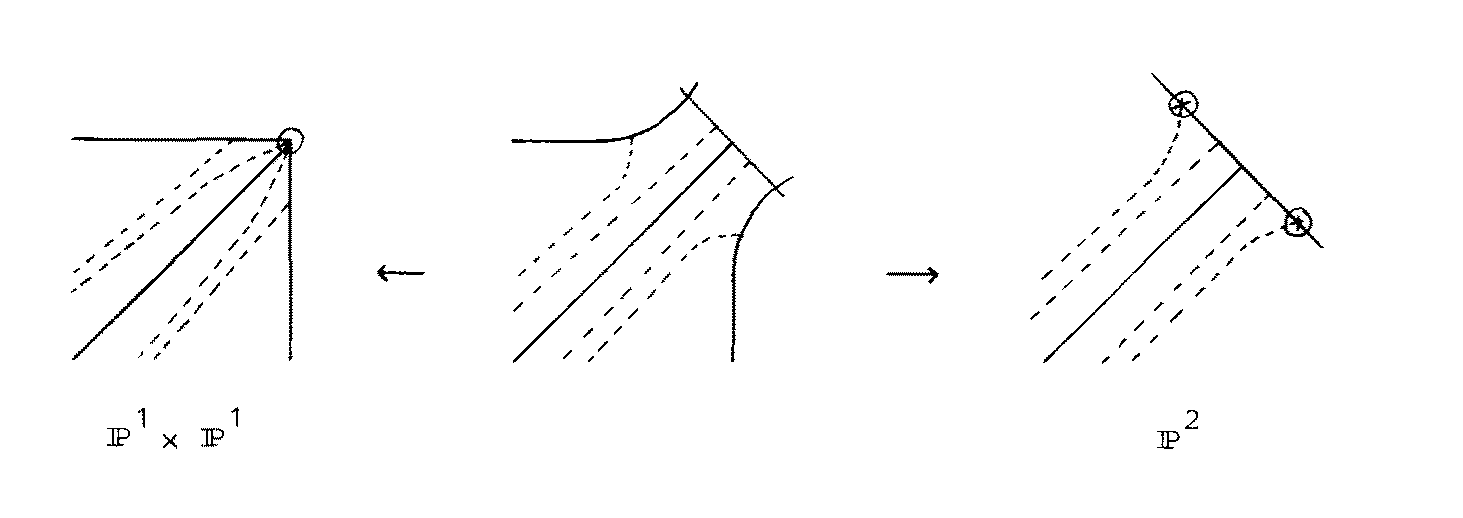
\includegraphics{assets/P08-A01_three_stage_compactification_present.png}\end{adjustbox}\end{center}
\noindent A similar construction can be made for arbitrary r and m.\par\smallskip
\noindent Return to the proof of 1.6. Apply 1.5 to h : Z \ensuremath{→} \ensuremath{\bar{B}}\allowbreak\_\ensuremath{α} and to \ensuremath{Δ}̄\allowbreak\_\ensuremath{α}. It follows that \ensuremath{Δ}̄\allowbreak\_\ensuremath{α} has an arbitrarily small open neighborhood \ensuremath{V_α} such that \ensuremath{h^{-1}}(\ensuremath{V_α}) = \ensuremath{h^{-1}}(\ensuremath{V_α} \ensuremath{∩} \ensuremath{B_α}) is connected and its \ensuremath{π₁} maps onto that of Z. By 1.7, whatever the neighborhood U of \ensuremath{Δ} in P, \ensuremath{V_α} can be chosen so that \ensuremath{V_α} \ensuremath{∩} \ensuremath{B_α} \ensuremath{⊂} U.\par\smallskip
\noindent The union V of the open subsets \ensuremath{V_α} \ensuremath{∩} \ensuremath{B_α} of P is an arbitrarily small neighborhood of \ensuremath{Δ}. Hypothesis b) on the \ensuremath{H_α} ensures that the intersection of the \ensuremath{V_α} \ensuremath{∩} \ensuremath{B_α} meets h(Z). Hence \ensuremath{h^{-1}}(V), a union of connected open subsets \ensuremath{h^{-1}}(\ensuremath{V_α}) with nonempty common intersection, is connected. Since the \ensuremath{π₁} of one of the \ensuremath{h^{-1}}(\ensuremath{V_α}) maps onto that of Z, a fortiori the same is true for \ensuremath{h^{-1}}(V), and this completes the proof.\par\smallskip
\noindent 2. Proof of Theorem 1\par\smallskip
\noindent 2.1.- Let C \ensuremath{⊂} \ensuremath{ℙ^2} be a reduced plane curve, let D be an irreducible component of C, let C' = \ensuremath{\overline{(C - D)}} be the union of the other components, let Sing(C) be the set of singular points of C, and let D* = D - Sing(C). Choose a base point O \ensuremath{∈} \ensuremath{ℙ^2} - C, and let \ensuremath{γ} be a loop in \ensuremath{ℙ^2} - C of the following type: \ensuremath{γ} goes from O along a path ch to a point p' near a point p of D*, goes once around D* in the positive direction, and returns to O along ch\textasciicircum{}\{-1\}. Since D* is connected, all loops of this type are conjugate. The quotient of \ensuremath{π₁}(\ensuremath{ℙ^2} - C,O) by the normal subgroup they generate is \ensuremath{π₁}(\ensuremath{ℙ^2} - C').\par\smallskip
\noindent PROPOSITION 2.2.- Suppose that the singular points of C lying on D are double points with distinct tangents. Then \ensuremath{γ} is central in \ensuremath{π₁}(\ensuremath{ℙ^2} - C,O).\par\smallskip
\noindent Let j be the inclusion of \ensuremath{ℙ^2} - C into \ensuremath{ℙ^2}, let g : \ensuremath{\widetilde{D}} \ensuremath{→} D be the normalization of D, and apply 1.6 to\par\smallskip
\noindent h = j \ensuremath{×} g : (\ensuremath{ℙ^2} - C) \ensuremath{×} \ensuremath{\widetilde{D}} \ensuremath{→} \ensuremath{ℙ^2} \ensuremath{×} \ensuremath{ℙ^2}.\par\smallskip
\noindent To describe conveniently the inverse images of certain neighborhoods of the diagonal, choose on \ensuremath{ℙ^2} a Riemannian structure such that, near each\par\smallskip
\end{minipage}
\end{adjustbox}
\newpage
\noindent\begin{adjustbox}{max totalsize={\textwidth}{0.945\textheight},center}
\begin{minipage}{\textwidth}
\noindent\hfill\scriptsize Authority physical page 9 / printed folio 543-09\par\normalsize
\noindent point P \ensuremath{∈} D \ensuremath{∩} Sing(C), \ensuremath{ℙ^2} is Euclidean and the two branches of C through P are orthogonal real 2-planes.\par\smallskip
\noindent If (u,v) \ensuremath{∈} (\ensuremath{ℙ^2} - C) \ensuremath{×} \ensuremath{\widetilde{D}} lies in the inverse image of a sufficiently small neighborhood of the diagonal, that is, if u and v are sufficiently close, then u is near D and one can drop a short perpendicular from u to D. When u is near Sing(D), there are even two such perpendiculars, one for each branch. Choose the one whose foot \ensuremath{\bar{u}} is close to v on \ensuremath{\widetilde{D}}:\par\smallskip
\begin{center}\begin{adjustbox}{max width=0.96\linewidth,max height=0.25\textheight}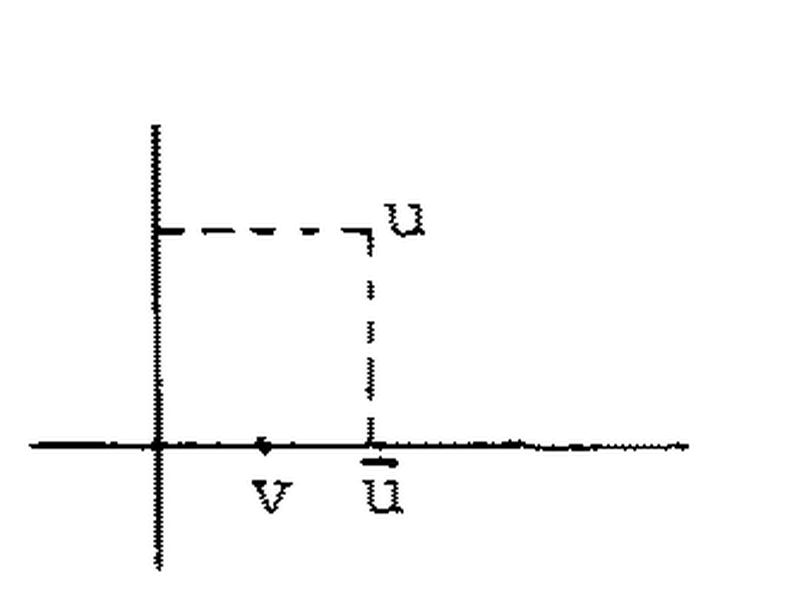
\includegraphics{assets/P09-A01_local_perpendicular_present.png}\end{adjustbox}\end{center}
\noindent The point \ensuremath{\bar{u}} lies in D*.\par\smallskip
\noindent Conversely, let \ensuremath{ε} > 0 be sufficiently small, and let q : U* \ensuremath{→} D* be the punctured-disk subbundle of the normal bundle of D* in \ensuremath{ℙ^2} consisting of nonzero normal vectors of length < \ensuremath{ε}. Let E be the set of pairs (x,v) with x \ensuremath{∈} U*, v \ensuremath{∈} \ensuremath{\widetilde{D}}, and d(q(x),v) < \ensuremath{ε} (distance measured on \ensuremath{\widetilde{D}}). The map pr\ensuremath{₁} : E \ensuremath{→} U* is a homotopy equivalence and has the space of pairs (x,q(x)) as a section. The map exp : (x,v) \ensuremath{↦} (exp(x),v) from E to (\ensuremath{ℙ^2} - C) \ensuremath{×} \ensuremath{\widetilde{D}} identifies E with the inverse image of a neighborhood of \ensuremath{Δ}, and as \ensuremath{ε} \ensuremath{→} 0 one obtains inverse images of a fundamental system of neighborhoods. Applying 1.6, one finds that for every O \ensuremath{∈} U*, exp and q induce a surjection\par\smallskip
\noindent (exp,q)* : \ensuremath{π₁}(U*,O) \ensuremath{↠} \ensuremath{π₁}(\ensuremath{ℙ^2} - C,exp(O)) \ensuremath{×} \ensuremath{π₁}(\ensuremath{\widetilde{D}},q(O)).\par\smallskip
\noindent There is an exact homotopy sequence\par\smallskip
\noindent \ensuremath{ℤ} \ensuremath{→} \ensuremath{π₁}(U*,O) \ensuremath{→} \ensuremath{π₁}(D*,q(O)) \ensuremath{→} 1.\par\smallskip
\noindent The image of \ensuremath{ℤ} is central; the image of 1 \ensuremath{∈} \ensuremath{ℤ} is represented by a small loop going once around D* in the positive direction. Since (exp,q)*, and hence exp* : \ensuremath{π₁}(U*,O) \ensuremath{→} \ensuremath{π₁}(\ensuremath{ℙ^2} - C,exp(O)), is surjective, this loop also defines a central element of \ensuremath{π₁}(\ensuremath{ℙ^2} - C,exp(O)). It is \ensuremath{γ}.\par\smallskip
\noindent 2.3 Proof of Theorem 1: For every irreducible component D of C, let \ensuremath{γ}(D) be the corresponding central element of \ensuremath{π₁}(\ensuremath{ℙ^2} - C,O). The quotient of \ensuremath{π₁}(\ensuremath{ℙ^2} - C,O) by the - central - subgroup generated by the \ensuremath{γ}(D) is \ensuremath{π₁}(\ensuremath{ℙ^2},O) = \{e\}. The theorem follows.\par\smallskip
\end{minipage}
\end{adjustbox}
\newpage
\noindent\begin{adjustbox}{max totalsize={\textwidth}{0.945\textheight},center}
\begin{minipage}{\textwidth}
\noindent\hfill\scriptsize Authority physical page 10 / printed folio 543-10\par\normalsize
\noindent BIBLIOGRAPHY\par\smallskip
\noindent [1] S. ABHYANKAR - Tame coverings and fundamental groups of algebraic varieties I, Amer. J. of Math., 81(1959), 46-94.\par\smallskip
\noindent [2] D. CHENIOT - Un théorème du type de Lefschetz, Annales de l'Institut Fourier, 25 1(1975), 195-213.\par\smallskip
\noindent [2 bis] D. CHENIOT - Une démonstration du théorème de Zariski sur les sections hyperplanes d'une hypersurface projective et du théorème de Van Kampen sur le groupe fondamental du complémentaire d'une courbe plane, Comp. Math., 27 2(1973), 141-158.\par\smallskip
\noindent [3] W. FULTON - On the fundamental group of the complement of a node curve, Ann. of Math., 111 2(1980), 407-409.\par\smallskip
\noindent [4] W. FULTON and J. HANSEN - A connectedness theorem for projective varieties, with applications to intersections and singularities of mappings, Ann. of Math., 109 1(1979), 159-166.\par\smallskip
\noindent [5] T. GAFFNEY and R. LAZARSFELD - On the ramification of branched coverings of \ensuremath{ℙ^n}, Inv. Math., 59 1(1980), 53-58.\par\smallskip
\noindent [6] H. HAMM et LÊ D\ensuremath{\widetilde{U}}NG TRANG - Un théorème de Zariski du type de Lefschetz, Ann. Sci. E.N.S., 6 3(1973), 317-366.\par\smallskip
\noindent [7] J.-P. SERRE - Revêtements ramifiés du plan projectif (d'après S. Abhyankar), Sém. Bourbaki 204, mai 1960.\par\smallskip
\noindent [8] O. ZARISKI - On the problem of existence of algebraic functions of two variables possessing a given branch curve, Amer. J. of Math., 51(1929), 305-328.\par\smallskip
\noindent [9] O. ZARISKI - Algebraic surfaces, second supplemented edition, Ergebnisse 61, Springer-Verlag.\par\smallskip
\noindent I have just received (1/10/80) a very fine account surveying the methods studied here, their variants, and their many applications: W. FULTON and R. LAZARSFELD - Connectivity and its applications in algebraic geometry.\par\smallskip
\noindent Pierre DELIGNE\\Institut des Hautes Etudes\\Scientifiques\\35 route de Chartres\\F-91440 BURES-SUR-YVETTE\par\smallskip
\end{minipage}
\end{adjustbox}
\end{document}
